%%%%%%%%%%%%%%%%%%%%%%%%%%%%%%%%%%%%%%%%%%%%%%%%%%%%%%%%%%%%%%%%%%%%%%%%%%%%%%%%%%
% 1
%%%%%%%%%%%%%%%%%%%%%%%%%%%%%%%%%%%%%%%%%%%%%%%%%%%%%%%%%%%%%%%%%%%%%%%%%%%%%%%%%%

\section{Breast Cancer Detection}

\subsection{Early Breast Cancer Detection Systems}

% todo: explain what are mammograms -> support for why it's hard for radiologists alone to make decisions based on mammograms
% limitations of radiologists

Breast cancer detection (BCD) using mammograms, and any form of cancer using medical imagery, relies on the conventional diagnoses of expert radiologists \cite{Osareh2010}. These diagnoses rest on the correct interpretation of the mammograms, which may be subject to errors due to the difficulty of correctly interpreting them \cite{Elter2009}. Indeed, mammograms are 2D images of 3D breasts that correspond to the superposition of breast tissue, which increases the difficulty for a radiologist to correctly analyse patterns as masses often naturally form due to this superposition \cite{Elter2009}.\\

To assist radiologists in their interpretations of mammograms, Computer-Assisted Detection/Diagnosis (CAD) software have been employed since the 1970s. However, pre-1990s CAD systems were very primitive and did not offer much more knowledge than the expert radiologists' knowledge. These unsophisticated ``expert'' systems consisted of manually processing and modelling pixels to construct rule-based systems that mainly used \textit{if-else-then} statements \cite{Litjens2017}, highlighting their inadequacy to learn how to recognise patterns that can be used to detect breast cancer.

\begin{figure}[ht]
\centerline{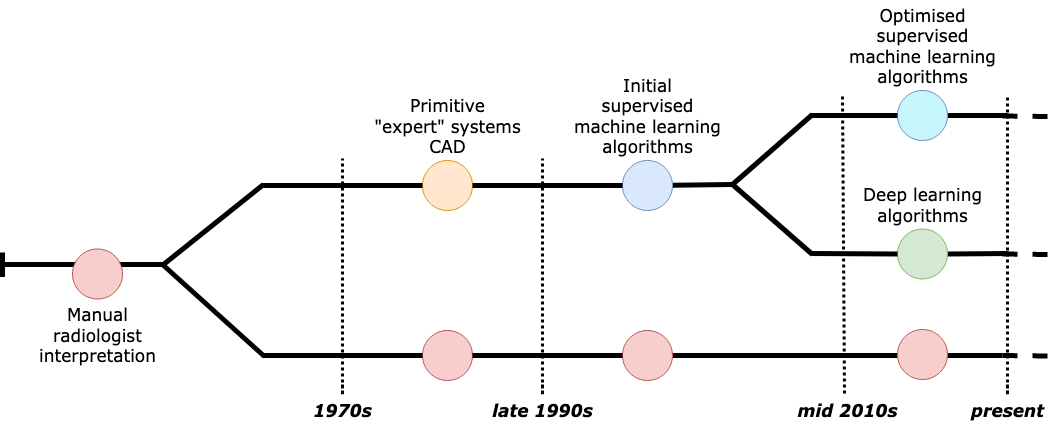
\includegraphics[width=\textwidth]{Dissertation/figures/litsurvey/bcd_timeline.png}}
\caption{\label{fig:litsurvey-bcd-timeline}Timeline of the evolution of breast cancer detection systems.}
\end{figure}

\subsection{Towards Supervised Machine Learning-based Systems}

Towards the late 1990s, supervised machine learning techniques started replacing these expert systems, allowing hidden patterns in the mammograms' data that could not be perceived by radiologists to now be recognised by these new algorithms. Machine learning-based approaches were selected over statistical approaches as they were more performant when dealing with large, complex and high-dimensional datasets \cite{Yue2018}, which is the case of datasets of mammograms. Additionally, machine learning methods were proven to be more suitable to the task of classification than traditional statistics-based approaches such as regression \cite{Paliwal2009}. This marked the shift from CAD systems that were fully designed by humans to systems that were trained on datasets of medical imagery \cite{Litjens2017}.\\

However, these machine learning models could not accurately operate on purely raw data such as the full-sized mammogram images. Indeed, all of the machine learning models tested against the task of breast cancer detection required relevant bits of information to be extracted first in order to solve the given task, such as k-Nearest Neighbour [kNN], Support Vector Machines [SVM], Decision Trees [DT], Naive Bayes [NB] and Artificial Neural Networks [ANN] \cite{Yue2018} \cite{Asri2016}. These important pieces of information pulled from the mammograms data correspond to features, and need to be extracted by humans before being fed to the aforementioned models for training. These features can range from colours, edges and corners to shapes and textures \cite{Geron2019}.\\

Logically, the next step in the evolution of breast cancer detection systems is for the model to learn these features on its own directly from the data rather than being fed hand-extracted features \cite{Yala2019}. Deep learning models, which corresponds to neural networks with hundreds of hidden layers, are based on this concept and are covered in Section~\ref{sec:litsurvey-DLtechniques-CNN}. However, these models have not been successfully implemented until recent years as they require powerful computers (usually equipped with Graphical Processing Units) to be efficiently trained. This means that nowadays, the machine learning models discussed in Section~\ref{sec:litreview-MLmodel-BCDapplications} still lead the field of breast cancer detection, with some manual mammogram interpretations still being carried out by radiologists \cite{Litjens2017}, as depicted in Figure~\ref{fig:litsurvey-bcd-timeline}.

% History of breast cancer detection (leads to)\\
% Motivation of using ML/DL for breast detection\\
% Problems with current breast cancer detection systems

%%%%%%%%%%%%%%%%%%%%%%%%%%%%%%%%%%%%%%%%%%%%%%%%%%%%%%%%%%%%%%%%%%%%%%%%%%%%%%%%%%
% 2
%%%%%%%%%%%%%%%%%%%%%%%%%%%%%%%%%%%%%%%%%%%%%%%%%%%%%%%%%%%%%%%%%%%%%%%%%%%%%%%%%%

\section{Machine Learning Models \& BCD Application}
\label{sec:litreview-MLmodel-BCDapplications}

\subsection{Machine Learning algorithms \& tasks}

\subsubsection{Types of learning algorithms}

Machine learning algorithms come in many flavours based on whether human supervision is required or not. The two main types of machine learning algorithms correspond to supervised and unsupervised learning. On the one hand in supervised learning, the dataset is labelled, meaning every sample in the dataset includes a solution \cite{Geron2019}. This label, often noted $y$, is used to make a prediction $\hat{y}$ by fitting the input features $\textbf{x}$ from a training dataset. The goal of a supervised learning algorithm is to determine the optimal parameters $\theta$ for the selected algorithm in order to minimise a loss function defined as $L(y,\hat{y})$, which corresponds to the error between the predicted algorithm's output $\hat{y}$ and the real output $y$ \cite{Litjens2017}. A large variety of loss functions can be used such as the general Mean Squared Error (MSE) and Mean Absolute Error (MAE) loss functions, or more specific loss functions such as the Hinge Loss for SVMs \cite{Geron2019}. The main applications of supervised learning are classification and regression, with the former being the most relevant to breast cancer detection.\\

On the other hand in unsupervised learning, the data is unlabelled, meaning only the input features $\textbf{x}$ are available while the labels $y$ are not \cite{Litjens2017}. This means the algorithm cannot optimise its hyperparameters by minimising a loss function. Instead, the algorithm needs to automatically create clusters in the dataset in order separate them into different groups. The main applications of unsupervised learning are clustering, anomaly detection, data visualisation and dimensionality reduction \cite{Geron2019}, rendering them irrelevant to the breast cancer detection. Two other types of machine learning exist, corresponding to semi-supervised learning and reinforcement learning, but are also irrelevant to the task of detecting breast cancer.\\

Among the aforementioned types of machine learning algorithms, the most pertinent one for the task of breast cancer detection is supervised learning as datasets of mammograms need to contain properly labelled data for each sample, indicating the status of the mammogram i.e. no tumour, benign tumour, malignant tumour \cite{Shen2017}.

\subsubsection{Machine learning BCD task}

\begin{itemize}
    \item Detection \& Classification
    \item Segmentation
    \item Other tasks: Briefly mention registration, CBIR, image generation, image enhancement. Regression?
\end{itemize}

\subsection{BCD Classification Models Comparison}

Since the late 1990s, a rich array of supervised machine learning algorithms have been applied and tested against the task of breast cancer detection, yielding varying results but ultimately contributing to improving accuracies for detecting breast cancer. The main types of algorithms used in breast cancer detection, which consist of k-Nearest Neighbour, Naive Bayes, Support Vector Machines, Decision Trees and Artificial Neural Networks, are briefly explained in the following sections before comparing their results to draw a picture of the advantages and disadvantages of each method.

\subsubsection{k-Nearest Neighbours}
\label{sec:litreview-knn}

kNN is one of the simplest machine learning algorithms and is often used as an initial benchmark when studying a dataset with no prior knowledge \cite{peterson2009k}. It is a non-parametric and lazy model, as it does not learn the data's pattern but rather classifies a test sample by looking at its $k$ nearest neighbours \cite{Yue2018}. These data point's nearest neighbours are determined by using distance metrics, with the Euclidian distance defined by Equation~\ref{eq:euclidian-distance} ($n$-dimensional space between two data points $s$ and $p$) being the preferred metric \cite{peterson2009k}. Figure~\ref{fig:litsurvey-knn-example} depicts an example of how a kNN classifier would distinguish between a benign and a malignant tumour using $k=3$.

\begin{equation}
\label{eq:euclidian-distance}
    d(s,p)=\sqrt{\sum_{i=1}^{n}(s_i-p_i)^2}
\end{equation}

\begin{figure}[ht]
\centerline{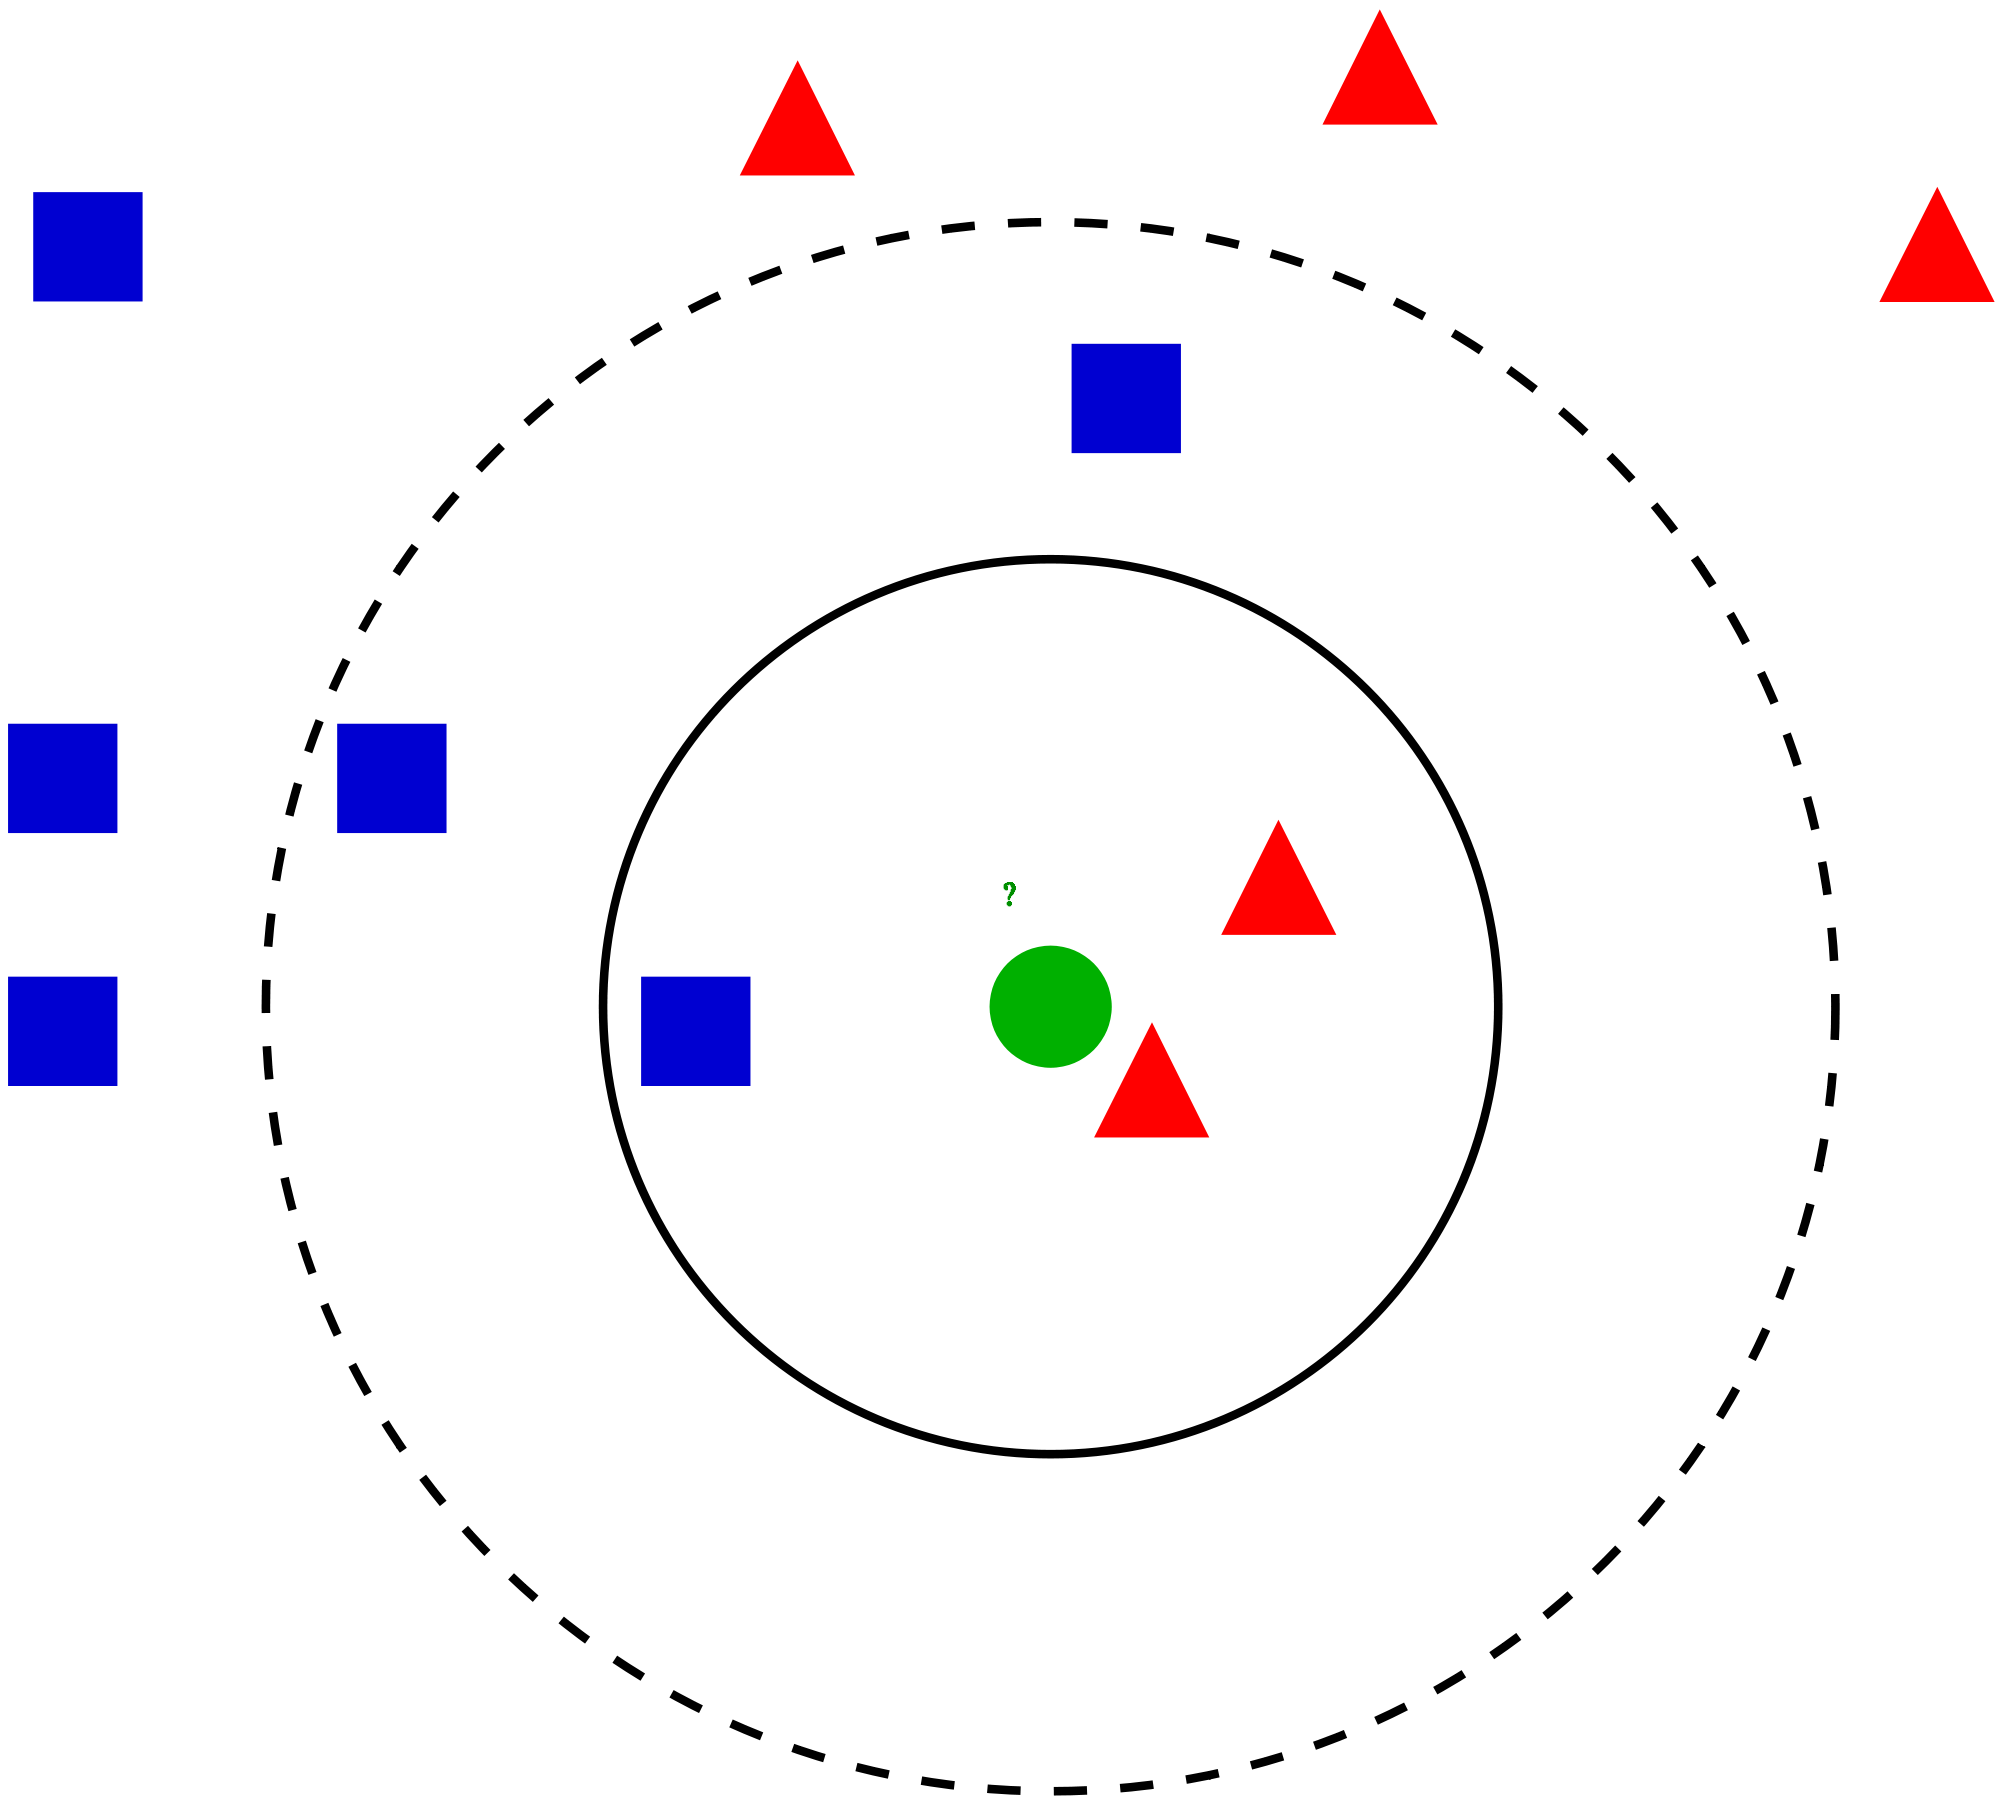
\includegraphics[width=0.4\textwidth]{Dissertation/figures/litsurvey/knn.png}}
\caption{\label{fig:litsurvey-knn-example}Example of a kNN classifier distinguishing between benign (blue square) and malignant (red triangle) tumours for a test data sample (green circle) using $k=3$. The test sample is classified as malignant as there are two red triangles and one blue square amongst the three neighbours. Figure retrieved online from T. Srivastava (\url{https://www.analyticsvidhya.com/blog/2018/03/introduction-k-neighbours-algorithm-clustering}).}
\end{figure}

Being generally used as an initial algorithm on new datasets, the kNN algorithm has often been tested on different datasets of mammograms for breast cancer detection, including the ``Wisconsin Breast Cancer Wisconsin Dataset (WBCD)'' \cite{Wolberg1995} and the ``Digital Database for Screening Mammography (DDSM)'' \cite{DDSMdataset2001} datasets. Despite all papers finding that a value of $k=1$ seemed to yield the most accuracy, a 1-NN classifiers often underperforms compared to other classifiers mentioned below, especially compared to SVMs and ANNs. Indeed, final model accuracies are on average 1-2\% lower than the most accurate solution found \cite{Yue2018} \cite{Asri2016} \cite{Montazeri2016}. Nevertheless, the results achieved by kNN are useful when used a basic benchmark against other models described below.

\subsubsection{Naive Bayes}

Naive Bayes uses Bayes' theorem and the assumption that all input features are independent from one another, which can be described as the input features $\textbf{x}=(\textbf{x}_1, ..., \textbf{x}_n)$ being independent given a class label $C$ in Equation~\ref{eq:naive-bayes} \cite{rish2001empirical}.

\begin{equation}
\label{eq:naive-bayes}
    P(\textbf{x}|C)=\prod_{i=1}^{n}P(\textbf{x}_i|C)
\end{equation}

This assumption leads to a naive model that despite not learning the data's underlying pattern (in a similar fashion to kNN), still offers competitive results in practice \cite{russell2002artificial}, notably in the field of medical imagery analysis \cite{rish2001empirical}. Naive Bayes achieves comparable accuracies to the aforementioned 1-NN classifiers, obtaining lower accuracies than the optimal algorithms found \cite{Yue2018} \cite{Montazeri2016}, but remaining useful for assessing basic benchmarks to compare with more advanced models discussed below.

\subsubsection{Decision Trees}

\textit{TODO: briefly describe DT and the C4.5 DT algorithm.}

\begin{figure}[ht]
\centerline{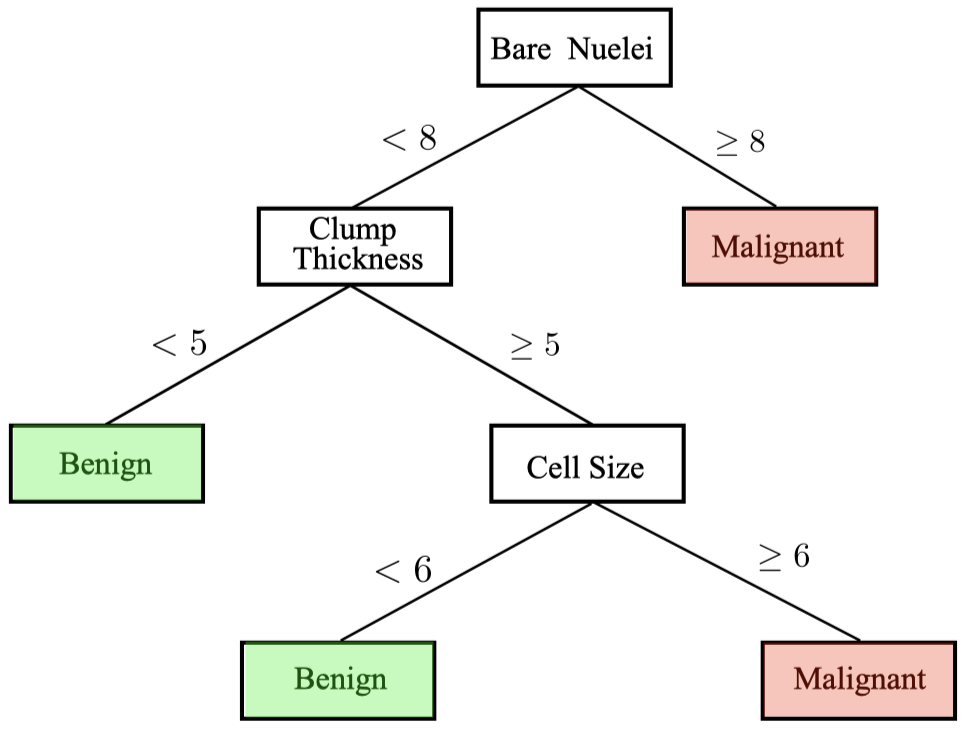
\includegraphics[width=0.65\textwidth]{Dissertation/figures/litsurvey/dt.png}}
\caption{\label{fig:litsurvey-dt-example}Example of a decision tree classifier distinguishing between benign and malignant tumours based on three extracted features from a dataset of mammograms: the size of the bare nuclei, the thickness of the clump and the uniformity of the cell size. Figure created by Yue et al. (2018).}
\end{figure}

C4.5 decision tree classifiers on their own did not offer better performances than kNN and NB classifiers, still falling short of the performance achieved by SVMs and ANNs \cite{Yue2018} \cite{Asri2016}. However, using C4.5 decision trees in hybrid systems that include SVMs and NBs produces accuracies akin to SVMs and ANNs \cite{Yue2018}.

\subsubsection{Support Vector Machines}

\textit{TODO: briefly describe SVM.}\\

\begin{figure}[ht]
\centerline{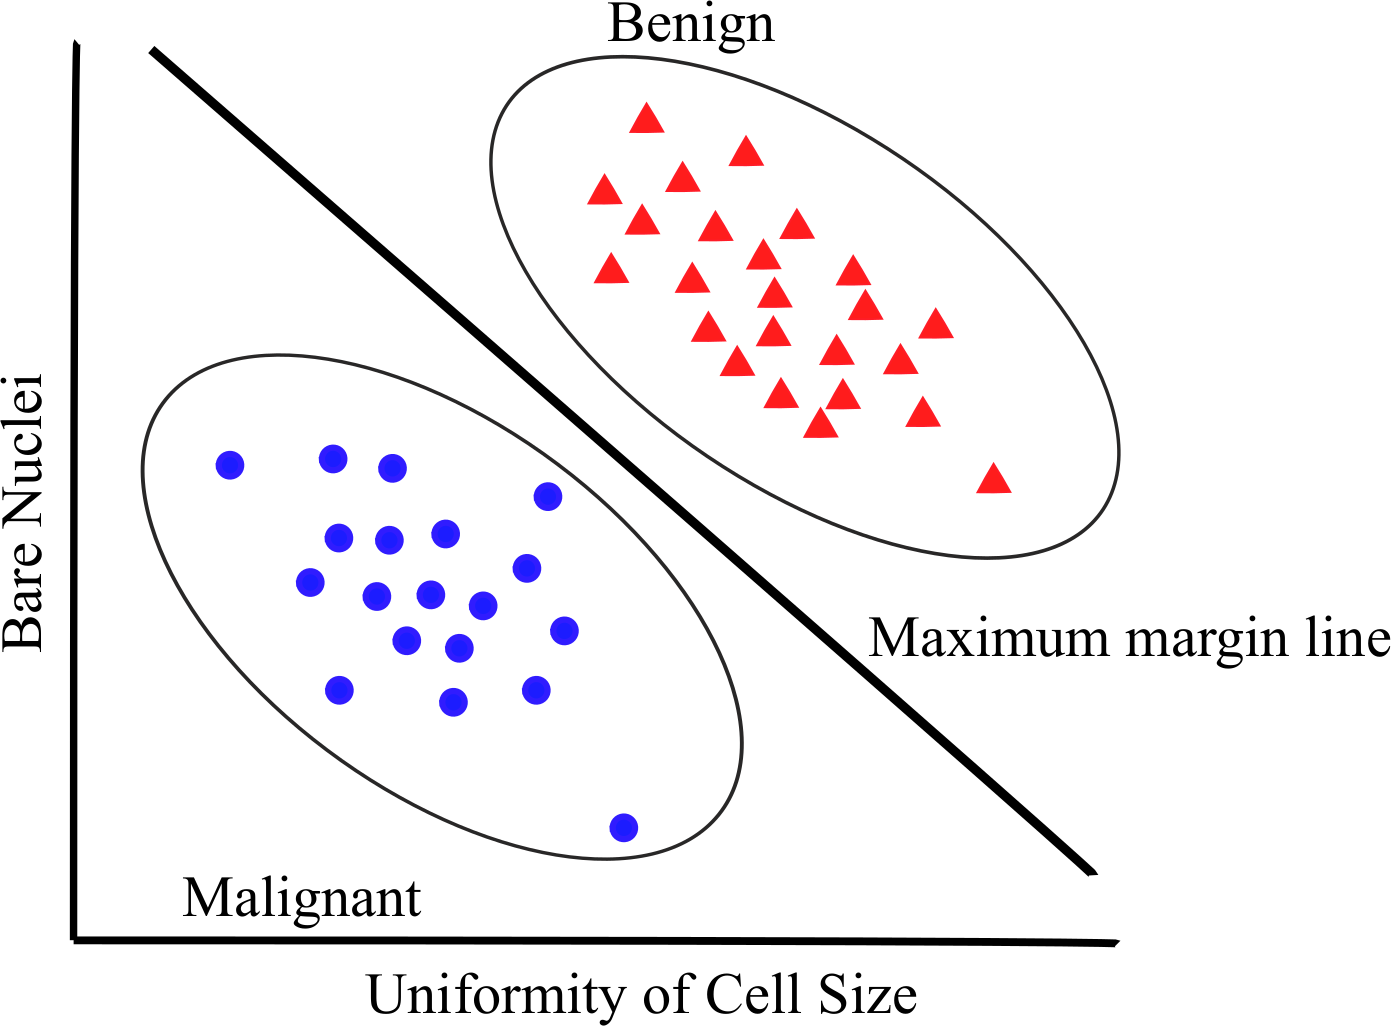
\includegraphics[width=0.6\textwidth]{Dissertation/figures/litsurvey/svm.png}}
\caption{\label{fig:litsurvey-svm-example}Example of a SVM classifier distinguishing between benign and malignant tumours based on two extracted features from a dataset of mammograms: the size of the bare nuclei and the uniformity of the cell size. Figure created by Yue et al. (2018).}
\end{figure}

SVMs with RBF kernels outperformed polynomial kernels \cite{Osareh2010}.

\subsubsection{Artificial Neural Networks}

\textit{TODO: briefly describe ANN.}

\begin{figure}[ht]
\centerline{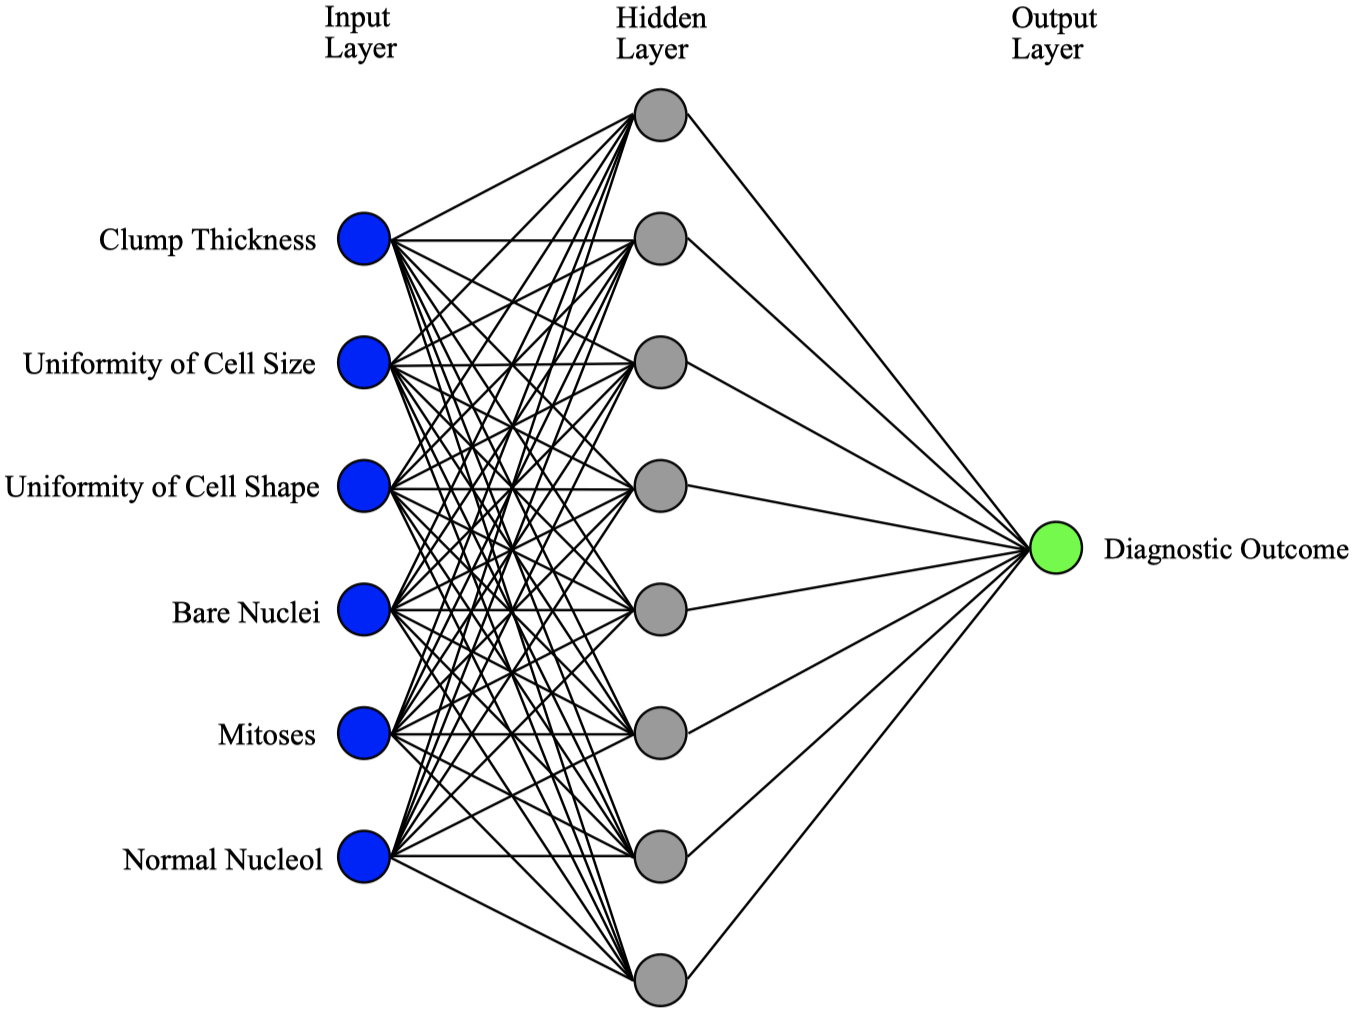
\includegraphics[width=\textwidth]{Dissertation/figures/litsurvey/ann.png}}
\caption{\label{fig:litsurvey-ann-example}Example of an ANN classifier distinguishing between benign and malignant tumours based on eight extracted features from a dataset of mammograms. Figure created by Yue et al. (2018).}
\end{figure}

\begin{itemize}
    \item Multi-Layer Perceptrons (shallow artificial neural networks)
    \item Deep neural networks
\end{itemize}

\textit{For each, mention pros and cons based on existing papers and compare different approaches. Naturally lead towards deep neural networks (e.g. CNNs) for the final section.}

\subsubsection{Machine learning algorithm comparison}

These algorithms heavily rely on the features extracted from the mammograms for classification. On their own, each algorithm's limitations prevent it from performing well on known datasets. However, combining them in hybrid systems increases the accuracy achieved, but greatly increases the algorithm's complexity.

%%%%%%%%%%%%%%%%%%%%%%%%%%%%%%%%%%%%%%%%%%%%%%%%%%%%%%%%%%%%%%%%%%%%%%%%%%%%%%%%%%
% 3
%%%%%%%%%%%%%%%%%%%%%%%%%%%%%%%%%%%%%%%%%%%%%%%%%%%%%%%%%%%%%%%%%%%%%%%%%%%%%%%%%%

\section{Deep Learning techniques \& CNNs}
\label{sec:litsurvey-DLtechniques-CNN}

\subsection{Convolution Neural Networks}

\begin{itemize}
    \item Deep Neural Networks
    \item Convolutional Neural Networks
\end{itemize}

Explore the techniques used in deep learning (techniques, databases, processing, libraries, output metrics, etc.)\\
Explore the deep learning model that will be explored by each dissertation

\subsection{Rise of Deep Learning in Medical Imagery Analysis}

\begin{itemize}
    \item Evolution of CNNs (first CNN used, first CNN applied to medical imagery analysis, famous architectures e.g. LeNet, AlexNet, GoogLeNet, ResNet, etc.)
    \item Transfer learning
    \item Hardware advances (GPUs)
    \item Software advanced (libraries)
\end{itemize}

\subsection{Current Limitations}

todo

%%%%%%%%%%%%%%%%%%%%%%%%%%%%%%%%%%%%%%%%%%%%%%%%%%%%%%%%%%%%%%%%%%%%%%%%%%%%%%%%%%
% 4 - CHAPTER SUMMARY
%%%%%%%%%%%%%%%%%%%%%%%%%%%%%%%%%%%%%%%%%%%%%%%%%%%%%%%%%%%%%%%%%%%%%%%%%%%%%%%%%%

\section{Chapter Summary}

Todo: review.
